\chapter{Teor\'ia de la aproximaci\'on de funciones}
\label{ch:approxTheory}

En los cursos b\'asicos de geometr\'ia anal\'itica y de c\'alculo diferencial se encuentra frecuentemente el problema de encontrar la recta que pasa por dos puntos dados (\textbf{puntos de control}).
Este es quiz\'as el ejemplo m\'as sencillo de interpolaci\'on: ajustar la curva que pasa por los puntos dados.

\begin{figure}[H]
\centering
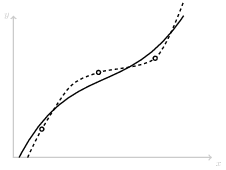
\includegraphics{approximationVSinterpolation}
\caption{Interpolaci\'on ( \protect\tikz \protect\draw[dashed, thick] (0,0) -- (0.6,0); ) y aproximaci\'on ( \protect\tikz \protect\draw[thick] (0,0) -- (0.6,0); ) de tres puntos de control.}
\label{f:ApproxVsIntepo} % APPROXimation Versus INTERPOlation
\end{figure}

Para el caso de datos experimentales, no se tiene la total certeza de la exactitud de los mismos por lo que una curva que se \textit{aproxime} bien podr\'ia modelar el fen\'omeno.
Adem\'as, se ha demostrado que en ciertos casos el interpolar puede resultar en comportamientos que difieren del esperado en el fen\'omeno, por ejemplo, la curva puede oscilar demasiado y no reproducir adecuadamente las formas deseadas (\autoref{f:lagrangeInterpolation}).
Se ha observado que en el caso de interpolaciones polinomiales, estas oscilaciones incrementan con la cantidad de datos, equivalentemente, con el grado del polinomio.
Por lo tanto, no importa cu\'antos puntos de control se agreguen, no hay garant\'ia de que los interpolantes polinomiales converjan a la curva o superficie que se quiere representar.

%La interpolaci\'on polinomial para muchos puntos es impr\'actica ya que el grado del interpolante puede ser demasiado alto lo cual conlleva a c\'alculos lentos y num\'ericamente inestables. 

\begin{figure}[H]
	\centering
	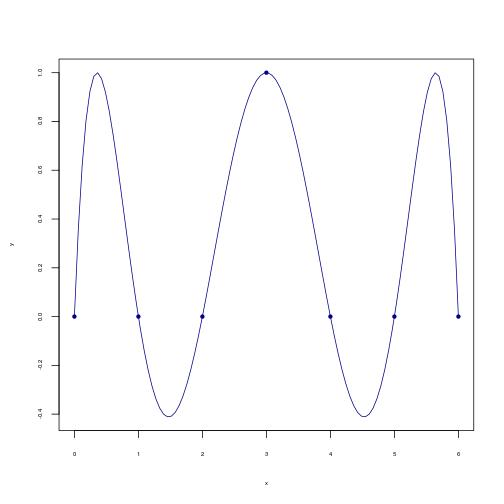
\includegraphics[width=0.6\textwidth]{LagrangeInterpolation-1}
	\caption{Interpolaci\'on de Lagrange.
	Observe las oscilaciones en la curva polinomial aun cuando no se observa tal oscilaci\'on en los puntos de control.}
	\label{f:lagrangeInterpolation}
\end{figure}

\section{Curvas de B\'ezier}
\label{s:bezier1D}

%La interpolaci\'on mediante splines (interpolaci\'on mediante funciones polinomiales por segmentos) es mejor computacionalmente porque ellos permiten mantener bajo el grado del polinomio. Pero sigue habiendo el mismo problema de oscilaci\'on. Por lo tanto se cambiar\'a de enfoque y se buscar\'a m\'etodos que permitan aproximar la forma descrita por puntos de control. No se insistir\'a que en la curva o superficie pase por los puntos de control, pero se har\'a \'enfasis en que las curvas capturen la forma definida por los puntos.

Un ejemplo de aproximaci\'on se forma al utilizar los polinomios de Bernstein, los cuales se definen de la siguiente manera \citep{goldman_pyramid_2002,phillips_interpolation_2003,mann_blossoming_2006,de_villiers_mathematics_2012}:

\begin{equation}
	B(u|i,n) = \binom{n}{i} u^i (1-u)^{n-i}
\end{equation}

\noindent
donde $u \in [0,1]$.

El conjunto de estos polinomios para una $n$ dada forma una base del espacio de polinomios de grado $n$. 

De esta manera, el teorema de Weiestrass establece que cualquier funci\'on continua se puede aproximar uniformemente mediante polinomios, en particular mediante las curvas de B\'ezier:

\begin{equation}
	B(u) = \sum_{i=0}^n P_i B(u|i,n)
\end{equation}

\noindent
donde $P_i \in \mathbb{R}^n$ son puntos de control tomados de la funci\'on a aproximar.

As\'i, se puede aproximar cualquier curva en $\mathbb{R}^n$. En el caso de puntos de control equiespaciados (\autoref{f:bezierFunc}) de la forma $(i/n, y_i)$, las curvas de B\'ezier presentan funciones de la forma $y = f(x)$:

\begin{align}
	B(u) &= \sum_{i=0}^n (i/n, y_i) B(u|i,n) \\
      &=  \left( u, \sum_{i=0}^n y_i B(u|i,n) \right)
\end{align}

Lo cual se puede re-escribir de la siguiente manera:

\begin{equation}
	B(u) = \sum_{i=0}^n
	f
	\left(
		\frac{i}{n}
	\right)
	B(u|i,n)
\end{equation}	

\begin{figure}[H]
	\centering 
	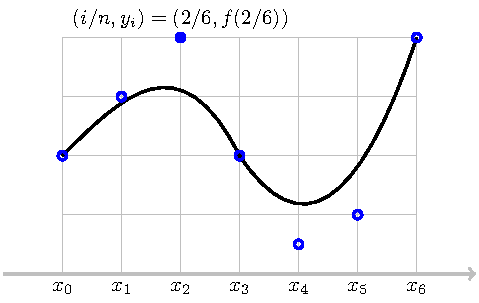
\includegraphics{bezierFunc}
	\caption{Curva de B\'ezier para el caso de puntos de control equiespaciados a lo largo del eje $x$.}
	\label{f:bezierFunc}
\end{figure}

Los polinomios de Bernstein-Kantorovich son un ejemplo de aplicaci\'on de esta \'ultima ecuaci\'on en la que se aproxima la funci\'on cuantil haciendo $f(i/n) = (x_{(i)} + x_{(i+1)})/2$ \citep[p. 392]{munoz-perez_estimating_1987}. Su implementaci\'on computacional se encuentra con el nombre \verb|dat2bernqua| dentro del paquete \href{https://cran.r-project.org/web/packages/lmomco/index.html}{\textit{lmomco}} del software estad\'istico \verb|R|.

Estas aproximaciones tienen muchas propiedades que la hacen populares en varios \'ambitos como en CAGD (Computer Aided Geometric Design) y en probabilidad con las c\'opulas de Bernstein.

Por ejemplo, si $f(x)$ es \textit{mon\'otona}, tambi\'en lo es su correspondiente curva de B\'ezier \citep[Theorem 7.1.2, p. 251]{phillips_interpolation_2003}. Ejemplo de funciones mon\'otonamente crecientes son las funciones de distribuci\'on de probabilidad.

\textit{Invarianza af\'in}. Se dice que una curva tiene invarianza af\'in si sus puntos de control viven en un espacio af\'in. Esta caracter\'istica garantiza que la curva sea independiente del sistema de coordenadas, y por lo tanto, una transformaci\'on af\'in de la curva solamente requiere transformar los puntos : $T(\sum_{k=0}^n P_k B(t|k,n))=\sum_{k=0}^nT(P_k)B(t|k,n)$.

\textit{Envolvente convexa (Convex Hull)}. Las curvas de B\'ezier siempre se encuentran dentro de la envolvente convexa de los puntos de control.
Esta propiedad garantiza que la curva est\'e ubicada en la proximidad de los puntos de control.
Adem\'as, tambi\'en garantiza que si los puntos de control son visibles en una pantalla, entonces la totalidad de la curva tambi\'en es visible (ver \autoref{f:BezierPropConvexHull}).

\begin{figure}[H]
	\centering
	\begin{subfigure}[b]{0.3\textwidth}
		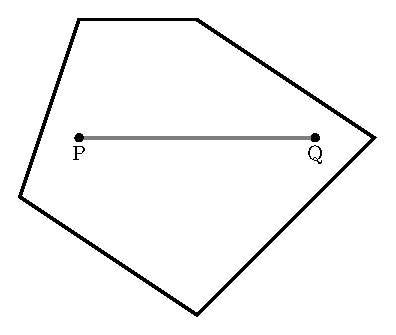
\includegraphics[width=\textwidth]{convexHull}
		\caption{Conjunto convexo.}
		\label{fig:convexHull}
	\end{subfigure} \qquad
	\begin{subfigure}[b]{0.3\textwidth}
		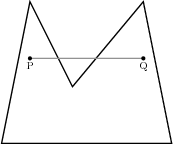
\includegraphics[width=\textwidth]{convexHullNon}
		\caption{Conjunto no convexo.}
		\label{fig:convexHullNon}
	\end{subfigure}
	\caption{Sean $P$ y $Q$ dos puntos en el conjunto $S \subset \mathbb{R}^n$. (a) El segmento rectil\'ineo $\overline{PQ}$ yace completamente dentro del conjunto convexo $S$; (b) Ejemplo que muestra un conjunto no convexo, en el cual parte del segmento rectil\'ineo yace fuera del conjunto.}
	\label{f:BezierPropConvexHull}
\end{figure}

\textit{Simetr\'ia}. Invertir el orden de los puntos de control produce la misma curva de B\'ezier, pero con orientaci\'on contraria.

\textit{Interpolaci\'on de los puntos extremos}. A diferencia de los polinomios de Lagrange, las curvas de B\'ezier generalmente no interpolan los puntos de control, pero siempre interpolan el primer y el \'ultimo punto.
Por ejemplo, un requisito de las funciones de distribuci\'on es que tome los valores $0$ y $1$ lo cual se da autom\'aticamente con los polinomios de Bernstein-B\'ezier.

\textit{No-degeneraci\'on}. Las curvas de B\'ezier son no-degeneradas, es decir, la curva nunca se colapsa un solo punto al menos que todos los puntos de control sean el mismo.

\textit{Derivada}. 
Si $F^{(k)}(x)$ definida en  $[0, 1]$ tiene un signo dado, entonces $B$ tiene el mismo signo en el mismo rango.
Por ejemplo, si $F(x)$ existe y es no-negativa, de tal manera que es convexa, entonces su correspondiente representaci\'on de B\'ezier satisface las mismas caracter\'isticas \citep[p. 254]{phillips_interpolation_2003}.
Adem\'as, si $F$ pertenece al espacio de las funciones con derivadas continuas hasta la $k$-\'esima derivada ($C_k[0, 1]$) para alg\'un entere $k \ge 0$, entonces $B^{(k)}$ converge uniformemente a $F^{(k)}$ \cite[p. 258]{phillips_interpolation_2003}.
Cuando $k = 1$ se tiene que $f(x)=F'(x)$, la densidad de probabilidad, es aproximada mediante la derivada de la curva de B\'ezier.

Esta propiedad tambi\'en explica que las curvas de B\'ezier preserven la forma de la curva.
La derivada se puede escribir como combinaci\'on lineal de dos polinomios de grado menor:

\begin{align}
	B'(u) &= n \sum_{i=0}^{n-1} (\Delta P_i) B(u|i, n-1) \\
	      &= n \sum_{i=0}^{n-1} (P_{i+1} - P_i) B(u|i,n-1)
\end{align}


Reescribi\'endola de otra manera:

\begin{equation}
	B'(u | P_0, \ldots, P_n) =
	n
	\left(
		B(u | P_0, \ldots, P_n) - 
		B(u | P_0, \ldots, P_{n-1})
	\right)
\end{equation}

\textit{Disminuci\'on de la variabilidad}. Intersecte una curva de B\'ezier en el plano con una l\'inea. Cuente el n\'umero de intersecciones entre la l\'inea y la curva $N_{lc}$ y entre la l\'inea y el pol\'igono de control $N_{lp}$. Esta propiedad asegura que  $N_{lc} \le N_{lp}$. Por ejemplo, si el pol\'igono de control oscila $w$ veces, entonces la curva no oscilar\'a m\'as que eso \citep{mann_blossoming_2006}.

\begin{figure}[H]
	\centering
		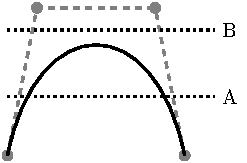
\includegraphics{variationDiminishing1}
		\qquad
		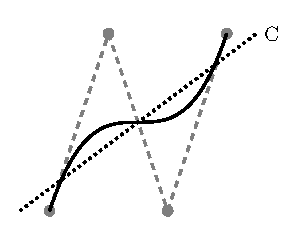
\includegraphics{variationDiminishing2}
		\qquad
		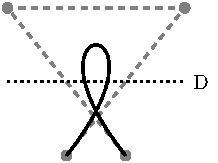
\includegraphics{variationDiminishing3}
		\label{fig:variationDiminishing3}
		\caption{Ilustraci\'on de la disminuci\'on en de la variabilidad de las curvas de B\'ezier para varios casos. L\'ineas negras punteadas que intersectan la curva de B\'ezier y sus puntos de control (en gris).}
	\label{fig:BezierPropVarDimi}
\end{figure}

Otra alternativa no param\'etrica, quiz\'as m\'as conocidas que las curvas de B\'ezier, son los splines, funciones polinomiales por tramos. Dentro de un contexto probabil\'istico, en \url{http://vita.had.co.nz/papers/density-estimation.pdf} se muestra una comparaci\'on de implementaciones con el enfoque de splines en el software estad\'istico \verb|R|.
